\documentclass[10pt]{beamer}
\usetheme[
%%% option passed to the outer theme
%    progressstyle=fixedCircCnt,   % fixedCircCnt, movingCircCnt (moving is deault)
  ]{Feather}
  
% If you want to change the colors of the various elements in the theme, edit and uncomment the following lines

% Change the bar colors:
%\setbeamercolor{Feather}{fg=red!20,bg=red}

% Change the color of the structural elements:
%\setbeamercolor{structure}{fg=red}

% Change the frame title text color:
%\setbeamercolor{frametitle}{fg=blue}

% Change the normal text color background:
%\setbeamercolor{normal text}{fg=black,bg=gray!10}

%-------------------------------------------------------
% INCLUDE PACKAGES
%-------------------------------------------------------

\usepackage[utf8]{inputenc}
\usepackage[english]{babel}
%\usepackage[francais, english]{babel}
\usepackage[T1]{fontenc}
\usepackage{helvet}
\usepackage{graphicx}


%-------------------------------------------------------
% DEFFINING AND REDEFINING COMMANDS
%-------------------------------------------------------

% colored hyperlinks
\newcommand{\chref}[2]{
  \href{#1}{{\usebeamercolor[bg]{Feather}#2}}
}

%-------------------------------------------------------
% INFORMATION IN THE TITLE PAGE
%-------------------------------------------------------

\title[] % [] is optional - is placed on the bottom of the sidebar on every slide
{ % is placed on the title page
      \textbf{Soutenance du travail encadré de recherche}
}

\subtitle[Moteur de présentation intéractif guidé par la voix]
{
	\textbf{Moteur de présentation intéractif guidé par la voix}
}

\author[Yemouna Manel CHIKBOUNI, Kévin LEBRETON, Thomas RAMBALDI]
{      Yemouna Manel CHIKBOUNI, Kévin LEBRETON, Thomas RAMBALDI
      %{\ttfamily lilqna.v@gmail.com}
}

\institute[]
{
	Faculté des sciences de Luminy\\
	Université d'Aix-Marseille\\
	Master 1 informatique\\
  
  %there must be an empty line above this line - otherwise some unwanted space is added between the university and the country (I do not know why;( )
}

\date{27 mai 2016}

%-------------------------------------------------------
% THE BODY OF THE PRESENTATION
%-------------------------------------------------------

\begin{document}

%-------------------------------------------------------
% THE TITLEPAGE
%-------------------------------------------------------

{\1% % this is the name of the PDF file for the background
% the plain option removes the header from the title page, noframenumbering removes the numbering of this frame only
\begin{frame}[plain,noframenumbering]
%Bonjour à toutes et à tous.
%Nous allons vous présentez notre projet.
%Tout d'abord une présentation de l'équipe de développement.
%Yemouna Manel Chikbouni, Kévin Lebreton et Thomas Rambaldi
%Notre tuteur et client est M. Béchet.
  \titlepage
\end{frame}


\begin{frame}{Table des matières}
%Donc tout d'abord nous allons vous faire une présentation du projet.
%Puis vous présentez, la méthode de travail utilisé employé
%Suivi du travail réalisé.
%Et pour finir une conclusion
	\tableofcontents
\end{frame}
}

%-------------------------------------------------------
%					Introduction
%-------------------------------------------------------
\section{Introduction}
\begin{frame}{Introduction}
%La présentation a pris différentes formes.
%Tout d'abord en écrivant au tableau, puis à l'aide des rétroprojecteurs et de fueille transparante, avec des vidéoprojecteur et à l'aide de claviers, souris. Ce qui peut-être un problème pour l'orateur.
%Toujours les mains prise ou déplacement forcé jusqu'à la machine.
%Présentation à venir grâce à cette application, pouvoir libérer le conférencier de ses mouvement, que cela soit de ses mains ou de ces déplacements. Ce qui apporte une présentation plus naturelle.
	\begin{block}{Les outils de présentations}	
		\begin{itemize}
			\item {\tt Les présentations avant}
			\item {\tt Les présentation de nos jours}
			\item {\tt Les présentation à venir grâce à cette application}
		\end{itemize}
	\end{block}
	\begin{center}
    	 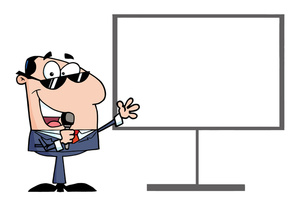
\includegraphics[width=5cm]{./images/presentation_voix}
	\end{center}
\end{frame}


%-------------------------------------------------------
%					Méthode de travail
%-------------------------------------------------------
\section{Méthode de travail}
\begin{frame}{Méthode de travail}
%Tout au long de ce projet nous avons travaillé avons la méthode agile.
%Celle-ci à pour but de prendre plusieurs rendez-vous pendant la phase du projet, qui consiste à plusieurs chose.
%Tout d'abord analysé le besoin.
%Puis recadrer si un hors sujet est faite
%Et enfin valider.
%Nous avons eu des réunions avec M. Béchet toutes les semaines pour la compréhension mais aussi pour lui montrer l'état d'avancement.
%Mais aussi avec M. Favre qui lui c'est de la partie au niveau des outils. Problème de fonctionnement ou non compréhension de ces derniers.
	\begin{block}{La méthode agile}
	  	\begin{itemize}
	  		\item {\tt Plusieurs réunions avec le client}
	  		\item {\tt Utile pour : }
			  	\begin{itemize}
	  				\item {\tt Analyser}
    					\item {\tt Recadrer}
    					\item {\tt Valider}
				\end{itemize}    		
    			
		\end{itemize}
	\end{block}
	
	\begin{block}{Organisation}
		\begin{itemize}
	  		\item {\tt Étude de projet}   		
    			\item {\tt Analyse des besoins}
    			\item {\tt Liste des différentes tâches}
    			\item {\tt Découpage des équipes}
    			\item {\tt Planning}
		\end{itemize}
	\end{block}
\end{frame}

%-------------------------------------------------------
%				Logiciel existant
%-------------------------------------------------------
%	  		\item {\tt Utilisé pour un spectacle}
%			  	\begin{itemize}
 %   					\item {\tt Crée des modèles de langage à partir d'un fichier XML}
%					\item {\tt Communication entre un client et un serveur}				
%				\end{itemize}
%			\item {\tt Permet de contrôler certains éléments du décors}
\section{Logiciel existant}
\begin{frame}{Logiciel existant}
	\begin{block}{Kaldi}
		\begin{itemize}		
			\item {\tt Logiciel de reconnaissance automatique de la parole}
			\begin{itemize}
    				\item {\tt Libre}			
			\end{itemize}
		\end{itemize}
	\end{block}
	
	\begin{block}{Homeostasis}
	  	\begin{itemize}
	  		\item {\tt Logiciel qui utilise une version modifiée de Kaldi}
	  		\begin{itemize}
    					\item {\tt Adapté pour un spectacle (Bruit ambiant)}
    					\item {\tt Adapté à l'accent espagnol des acteurs parlant anglais}	
			\end{itemize}
		\end{itemize}
	\end{block}
\end{frame}

%-------------------------------------------------------
%				Reconnaissance vocale
%-------------------------------------------------------
%\section{Reconnaissance vocale}
\begin{frame}{Logiciel existant}{Reconnaissance vocale}

	\begin{block}{Fonctionnement}
	  	\begin{itemize}
	  		\item {\tt Modèles acoustiques}
	  		\item {\tt Modèles lexicaux}
	  		\item {\tt Modèles de langage}
		\end{itemize}
	\end{block} 
	\begin{center}
	 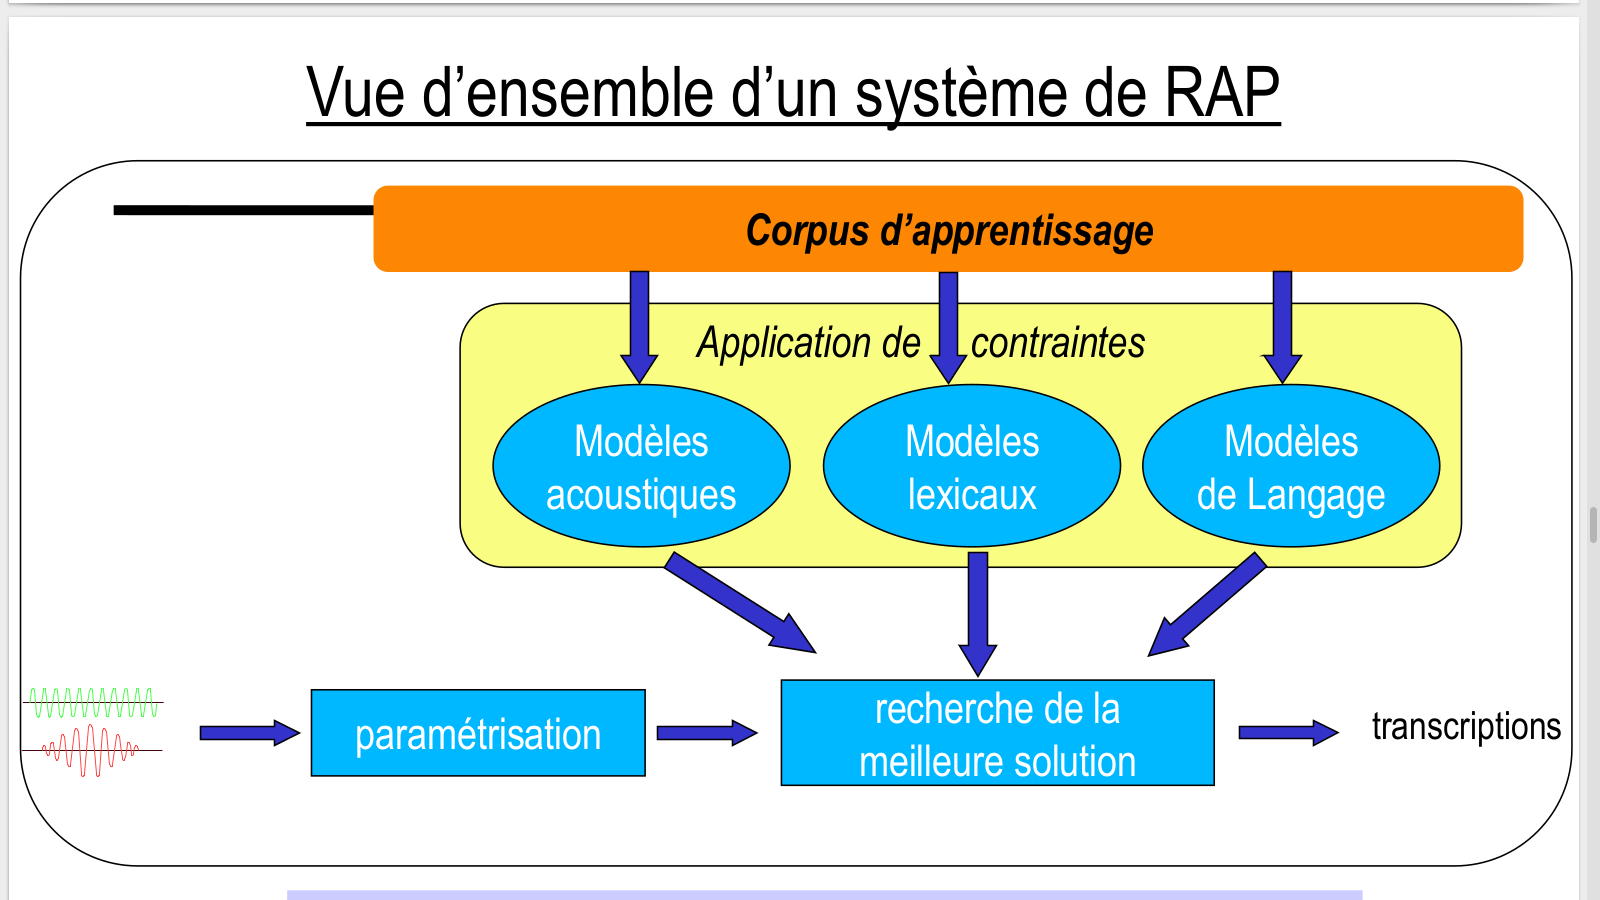
\includegraphics[width=9cm]{./images/reco_vocale}
	\end{center}
\end{frame}

%-------------------------------------------------------
%				SmartPrésentation
%-------------------------------------------------------

%	\begin{block}{Structure du projet <------}
%	  	\begin{itemize}
%	  		\item {\tt Kaldi}
%	  		\item {\tt XML}
%	  		\item {\tt Client/Serveur}
%	  		\item {\tt Interface graphique}	
%		\end{itemize}
%	\end{block}
	
\section{SmartPrésentation}
\begin{frame}{SmartPrésentation}{Présentation de l'application}
	\begin{block}{Outils utilisés}
	  	\begin{itemize}
	  		\item {\tt Kaldi}
	  		\item {\tt Homeostasis (Création de modèle de langage anglais)}
	  		\item {\tt Outil de création de modèles de langage français}
		\end{itemize}
	\end{block}	
	
	\begin{block}{Outils développés}
	  	\begin{itemize}
	  		\item {\tt Visualiseur de présentation}
	  		\item {\tt Communication entre un client et un serveur}
	  		\item {\tt Outil de création de fichier XML pour Homeostasis}
		\end{itemize}
	\end{block}		

\end{frame}

%\section{Plusieurs versions}
\begin{frame}{SmartPresentation}{Différentes versions}
%En ce qui concerne les différentes versions trois ont été développés.
%La première changement de diapositive en passant à la suivante ou à la précedante à l'aide deux de mots clé, comme next et previouis.
%Cette version comme l'avantage qu'elle est simple et répond au besoins du clients.
%Pour ce qui est des incovénients, il faut répéter que ces deux mots pour que la transition s'opère.
%Si le conférencier veux passer de la page trois à quinze, celui-ci doit répéter douze fois le mot next.
	\begin{block}{Version 1}
	  	\begin{itemize}
	  		\item {\tt Utilisation de deux mots-clés : Suivant / Précédent} 		
		\end{itemize}
	\end{block}

%Une fois la première version fonctionnelle, une amélioration a été apporté.
%Pour remédier a ces deux mots clés, chaque diapositive comporte son propre mot-clé pour passer à la diapositive suivante.
%Le mot-clé permettant de faire précédant n'existe plus.
%Pour faire un retour en arrière il faut que l'orateur prononce une séquence de mots-clé.
%Comme par exemple go to the slide plus le tire de la diapositive.
%Cette méthode permet bien éventullement d'aller à n'importe qu'elle diapositive se trouvant dans la présentation.
%Comme aller de la diapositive une à cinq.
%Cette amélioration apporte les avantages suivantes.
%Permet de naviguer entre n'importe qu'elle diaposive sans passer par les pages intermédiare
%Les désavantages, l'orateur doit se souvenir des tous les mots, c'est-à-dire tous les tires des diapositives.
	\begin{block}{Version 2}
	  	\begin{itemize}  
	  		\item {\tt Utilisation des titres des diapositives comme mots-clés}   		
		\end{itemize}
	\end{block}

%Enfin une derniere, où il a été implémenté un point supplémentaire.
%Ce point consiste à changer de diapositive à l'aide du texte.
%Pour que le changement s'opère, l'orateur prononce son texte.
%Dès que le système détecte un certain pourcentage du message qui est en concordance avec le texte inscrit dans le fichier Beamer, le changement se fait.
%Ce dernière version porte les avantages que l'orateur na plus besoin de se souvenir de chaque mot clé associé à la diapositive courante
%Mais il doit pour cela prononcer son texte qui est le plus proche prossible de celui qui a écrit au préalablement.
%Dans le cas où le présentation à un trou de mémoire, il peu utliliser le clavier en cas de secours.
%Ce qui permet d'éviter tout blocage lors d'une présentation.
	\begin{block}{Version 3}
	  	\begin{itemize}
    			\item {\tt Automatisation du changement de diapositive}
		\end{itemize}
	\end{block}
\end{frame}


%-------------------------------------------------------
%				Méthode de travail
%-------------------------------------------------------
\section{Travail effectué}
%-------------------------------------------------------
%				Beamer/XML
%-------------------------------------------------------
%	\begin{block}{Concernant les fichiers Beamer et XML}
%	  	\begin{itemize}
%	  		\item {\tt Lecture du fichier Beamer}
%	  		\item {\tt Écriture du fichier XML}
%	  		\item {\tt Lecture du fichier XML}
%		\end{itemize}
%	\end{block}
%\subsection{Beamer/XML}
\begin{frame}{Travail effectué}{LateX/XML}
	
	\begin{columns}
		\begin{column}{0.5\textwidth}
			\begin{block}{Pour la version anglaise}
				\begin{itemize}
					\item {\tt Lecture du fichier LateX}
	  				\item {\tt Construction du fichier XML}
				\end{itemize}
			\end{block}
		\end{column}
		
		\begin{column}{0.5\textwidth}
			\begin{block}{Pour la version française}
				\begin{itemize}
					\item {\tt Lecture du fichier LateX}
	  				\item {\tt Construction d'un fichier texte}
				\end{itemize}
			\end{block}
		\end{column}
	\end{columns}	
	
	\begin{block}{Outils utilisés}
		\begin{itemize}
			\item {\tt LateX}
			\item {\tt Bibliothèques : JDOM}
		\end{itemize}
	\end{block}		  			
\end{frame}


%-------------------------------------------------------
%				Client/Serveur
%-------------------------------------------------------
%\section{Client/Serveur}
\begin{frame}{Travail effectué}{Client/Serveur}
	\begin{block}{Client}
	  	\begin{itemize}
	  		\item {\tt En Python}
	  		\item {\tt Transmet la voix détectée par Kaldi}		
		\end{itemize}
	\end{block}


	\begin{block}{Serveur}
	  	\begin{itemize}
	  		\item {\tt En Java}
	  		\begin{itemize}
	    			\item {\tt Portabilité du code}
	    			\item {\tt Bibliothèques}
	    			\item {\tt Javadoc}
			\end{itemize}
			\item {\tt Analyse la voix reçue}	    		
		\end{itemize}
	\end{block}
	
	\begin{block}{Outils utilisés}
		\begin{itemize}
	    		\item {\tt JavaOSC}
		\end{itemize}
	\end{block}	
		  			
\end{frame}


%-------------------------------------------------------
%				Interface graphique
%-------------------------------------------------------
%\section{Interface graphique}
\begin{frame}{Travail effectué}{Interface graphique}
	\begin{block}{Ressemble aux visualiseurs existant}
	  	\begin{itemize}
	    		\item {\tt Plein écran}
	    		\item {\tt Changement de diapositives avec le clavier}
	    		\item {\tt Zoom}
		\end{itemize}
	\end{block}

	\begin{block}{Outils utilisés}
	  	\begin{itemize}
	    			\item {\tt Swing}
	    			\item {\tt JavaFX}	    		
			    \item {\tt PDFRenderer}		
		\end{itemize}
	\end{block}		  			
\end{frame}

%-------------------------------------------------------
%					Démonstration
%-------------------------------------------------------
\section{Démonstration}
\begin{frame}{Démonstration avec mot-clé}
%Cette démonstration va fonctionner avec le mot-clé : passer à la diapositive suivante	
	Cette démonstration va fonctionner avec le mot-clé : passer à la diapositive suivante	
\end{frame}

\begin{frame}{Démonstration pour aller sur une diapositive}
%Cette démonstration va fonctionner avec le mot-clé : "aller à la diapositive plusieurs versions"	
	Cette démonstration va fonctionner avec le mot-clé : "aller à la diapositive introduction"		
\end{frame}

\begin{frame}{Démonstration avec le texte}
%Dans cette partie de la démonstration, nous allons tester de passer à la diapositive suivante sans mot-clé, mais seulement avec le texte que je suis en train de lire
%Ce qui devrait nous mener à la diapositive concernant les perspectives
	Dans cette partie de la démonstration, nous allons essayer de passer à la diapositive suivante sans mot-clé, mais seulement avec le texte que je suis en train de lire. \\	
	
	Ce qui devrait nous mener à la diapositive concernant les perspectives
\end{frame}


%-------------------------------------------------------
%					Perspectives
%-------------------------------------------------------
\section{Perspectives}
\begin{frame}{Perspectives}
		
\includegraphics[width=1cm]{./images/idee}
	  	\begin{itemize}
			\item {\tt Créer une version éducative pour les enfants}
			\item {\tt Étendre cette application à d'autres logiciels de présentation}
			\item {\tt Créer plus d’interactions avec l'utilisateur }
		\end{itemize}
\end{frame}

%-------------------------------------------------------
%					Bilan Personnel
%-------------------------------------------------------
\section{Bilan Personnel}
\begin{frame}{Bilan Personnel}
	\begin{itemize}
		\item {\tt Travail avec la méthode agile}
		\item {\tt Développement des connaissances}
		\item {\tt Mise en application des connaissances acquises}	
		\item {\tt Découverte de nouveaux outils}
		\item {\tt Difficultés dans la mise en place du client/serveur}
		\item {\tt Difficultés dans les phases de tests}
		\item {\tt Difficultés dans la gestion de projet}
	\end{itemize}
\end{frame}

%-------------------------------------------------------
%					Conclusion
%-------------------------------------------------------
\section{Conclusion}
%\subsection{Loading the Theme and Theme Options}
\begin{frame}{Conclusion}
%Ce T.E.R. consistait à réaliser un moteur intéractif guidé par la voix pour faciliter l'intéraction entre le locuteur et sa présentation.
%A l'heure actuelle, l'application est prête à être utilisée. On  peu donc affirmer que le but qui avait été fixé est atteint.
%Certains points sont à améliorer. Comme la mise en place d'un système qui détecte lorsque l'orateur à finit sa diapositive afin qu'il change automatiquement.
%---->Parler des amélioration possible pour rendre l'application plus performante<-----
%Ce projet fonctionne est répond au besoin 	
%Ce T.E.R. à permis à tous les membres du groupes de mettre en application les compétences scolaire acquises et de les approfondir.
 	
	  	\begin{itemize}
			\item {\tt Apport du T.E.R. }
			\item {\tt Objectif atteint aux niveaux des besoins }
			\item {\tt Améliorer le projet }
			\item {\tt Cette présentation a été présenté avec l'application}
		\end{itemize}

\end{frame}


{\1
\begin{frame}[plain,noframenumbering]
%Nous vous remercions de votre attention, y a t-il des questions ?
  \finalpage{Merci pour votre attention}
\end{frame}
}

%-------------------------------------------------------
%					Références
%-------------------------------------------------------
\fontsize{7pt}{8}\selectfont
\begin{frame}{Références}
Kaldi : http://kaldi-asr.org 
\newline \\

Homeotasis : Speech Input for Live Performance : An Impromptu Dialogue Between the Computer and the Artist\\
Auteur : \textit{Benoît Favre, Mickael Rouvier, Frédéric Béchet and Rocio Berenguer}
\newline \\

Schéma : Vue d'ensemble d'un système de RAP\\
Auteur : Frédéric Béchet 
\newline \\

Logiciel de création de modèles de langage français\\
Auteur : \textit{Benoît Favre}
\end{frame}

\end{document}
